% A21SequencesAndSeriesTikZ-001.tex
% Asset ID: A21SequencesAndSeriesTikZ-001
% Purpose: Arithmetic series reverse-pairing proof.
\documentclass[tikz,border=10pt]{standalone}
\usetikzlibrary{arrows.meta,decorations.pathreplacing}
\begin{document}
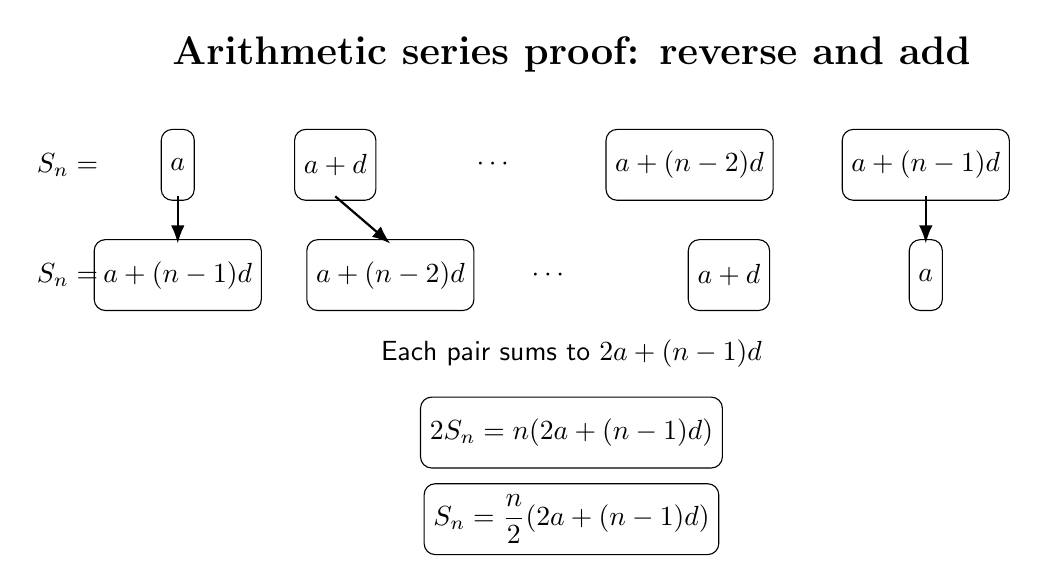
\begin{tikzpicture}[every node/.style={font=\sffamily},box/.style={draw,rounded corners,minimum height=0.9cm,align=center}]
\node[font=\bfseries\Large] at (6,3.6){Arithmetic series proof: reverse and add};
\node at (-0.4,2.2){$S_n=$};
\node[box] at (1,2.2){$a$};\node[box] at (3,2.2){$a+d$};\node at (5,2.2){$\cdots$};\node[box] at (7.5,2.2){$a+(n-2)d$};\node[box] at (10.5,2.2){$a+(n-1)d$};
\node at (-0.4,0.8){$S_n=$};
\node[box] at (1,0.8){$a+(n-1)d$};\node[box] at (3.7,0.8){$a+(n-2)d$};\node at (5.7,0.8){$\cdots$};\node[box] at (8,0.8){$a+d$};\node[box] at (10.5,0.8){$a$};
\draw[-{Latex},thick] (1,1.8)--(1,1.2);\draw[-{Latex},thick] (3,1.8)--(3.7,1.2);\draw[-{Latex},thick] (10.5,1.8)--(10.5,1.2);
\node at (6,-0.2){Each pair sums to $2a+(n-1)d$};
\node[box] at (6,-1.2){$2S_n=n(2a+(n-1)d)$};
\node[box] at (6,-2.3){$\displaystyle S_n=\frac n2(2a+(n-1)d)$};
\end{tikzpicture}
\end{document}
